% CVPR 2022 Paper Template
% !TEX root = PaperForReview.tex
\documentclass[12pt,letterpaper]{article}

\usepackage{cvpr}
\usepackage{titling}
\usepackage{enumitem}
\usepackage{graphicx}
\usepackage{amsmath}
\usepackage{amssymb}
\usepackage{booktabs}
\usepackage{CJKutf8}
\usepackage{geometry}
\usepackage{float}
 \geometry{
 a4paper,
 total={170mm,257mm},
 left=20mm,
 top=20mm,
 }
%  \setlength{\headheight}{15.0pt}
\addtolength{\topmargin}{-3.0pt}

\usepackage[pagebackref,breaklinks,colorlinks]{hyperref}
% \usepackage{fancyhdr}
% \fancypagestyle{plain}{%  the preset of fancyhdr 
%     \fancyhf{} % clear all header and footer fields
%     \fancyhead[L]{Computer Vision Homework 1 Report}
%     \fancyhead[R]{\today}
% }
\makeatletter
% Support for easy cross-referencing
\usepackage[capitalize]{cleveref}
\crefname{section}{Sec.}{Secs.}
\Crefname{section}{Section}{Sections}
\Crefname{table}{Table}{Tables}
\crefname{table}{Tab.}{Tabs.}
\newcommand{\xeq}[1]{Eq.~(\ref{#1})}
\newcommand{\xeqs}[2]{Eqs.~(\ref{#1}) and~(\ref{#2})}
\newcommand{\xkw}[1]{\textcolor{blue}{\textbf{#1}}}
\newcommand{\xfig}[1]{Figure~\ref{#1}}
\newcommand{\xfigx}[2]{Figures~\ref{#1}--\ref{#2}}
\newcommand{\xfigs}[2]{Figures~\ref{#1} and~\ref{#2}}
\newcommand{\xfigss}[3]{Figures~\ref{#1}, \ref{#2}, and~\ref{#3}}
\newcommand{\xfigsss}[4]{Figures~\ref{#1}, \ref{#2}, \ref{#3}, and~\ref{#4}}
\newcommand{\xsubfig}[1]{Figure~\ref{#1}}
\newcommand{\xsubfigs}[1]{Figures~\ref{#1}}
\newcommand{\xtab}[1]{Table~\ref{#1}}
\newcommand{\xtabs}[2]{Tables~\ref{#1} and~\ref{#2}}
\newcommand{\xtabss}[3]{Tables~\ref{#1}, ~\ref{#2}, and~\ref{#3}}
\newcommand{\xtabt}[2]{Tables~\ref{#1} through~\ref{#2}}
\newcommand{\xsec}[1]{Section~\ref{#1}}
\newcommand{\xalg}[1]{Algorithm~\ref{#1}}
\newcommand{\xalgs}[2]{Algorithms~\ref{#1} and~\ref{#2}}
\newtheorem{dpd}{Definition}
\newtheorem{xdefinition}{Definition}
\newcommand{\opt}{\mathop{\rm optimize}}
\newcommand{\subject}{\mathop{\rm subject~to}}
\newcommand{\xdf}[1]{Definition~\ref{#1}}

\newcommand{\xmetah}{metaheuristic}
\newcommand{\xmetahs}{metaheuristics}
\newcommand{\xmetaha}{metaheuristic algorithm}

\newcommand{\xPropose}{AdaMMP}
\newcommand{\xProposeFull}{Adaptive Multi-Metric Predictor}
\newcommand{\xProposeP}{\xPropose~proxy}
\newcommand{\xNAS}{neural architecture search}
\newcommand{\xnasblol}{NAS-bench-101}
\newcommand{\xnasbtss}{NAS-bench-201}
\newcommand{\xnasbsss}{NATS-bench-SSS}

\newcommand{\xq}[1]{\textcolor{red}{#1}}
\newcommand{\xqq}[1]{\textcolor{red}{\sout{#1}}}
% \newcommand{\xr}[1]{\label{#1}\textcolor{red}{(#1)}}
\newcommand{\xr}[1]{\label{#1}}
% \newcommand{\xs}[1]{\textcolor{magenta}{#1}}
\newcommand{\xs}[1]{#1}
\newcommand{\xt}[1]{\textcolor{black}{#1}}
\newcommand{\xx}[2]{{#2}}

\usepackage[normalem]{ulem}
\newcommand{\xold}[1]{\textcolor{red}{#1}} % original text
\newcommand{\xnew}[1]{\textcolor{blue}{#1}} % replacement text
\newcommand{\xch}[2]{\xqq{#1} \xnew{#2}}

% \newcommand{\xfig}[1]{圖~\ref{#1}}
% \newcommand{\xfigs}[2]{圖~\ref{#1} and~\ref{#2}}
% \newcommand{\xq}[1]{\textcolor{red}{#1}}

% \newcommand{\xmold}[1]{\textcolor{red}{#1}} % original text
% \newcommand{\xmnew}[1]{\textcolor{blue}{#1}} % replacement text
% \newcommand{\xch}[2]{\xmold{\sout{#1}}\xmnew{#2}}

\newcommand{\xAns}{\vskip 2mm\textbf{Answer:} }
\begin{document}
\begin{CJK}{UTF8}{bkai}
    %%%%%%%%% TITLE
    \title{Term Project Proposal - Co-Evolutionary Strategy Optimization for Multi-Agent Dodgeball Using Genetic Algorithms in a Dynamic 2D Environment}
    
    \author{
        Leader\\
        高聖傑\\
        313552011\\
        rabbitkao402@gmail.com
    }

    \maketitle
\end{CJK}

\section{Project Category}
Evolutionary computation application with a focus on co-evolutionary algorithm design.

\section{Objectives}
\subsection{Develop Effective Dodging and Throwing Strategies}
A simulation will be implemented to mimic a dodgeball game with two opposing teams: a dodging team and a throwing team.
Co-evolutionary Genetic Algorithms will be utilized to evolve strategies for both teams, from simple reactive behaviors to optimized movement, positioning, and decision-making, making sure the agents adapt to changing game dynamics effectively.

\subsection{Demonstrate Co-Evolutionary Dynamics}
Explore how competitive co-evolution can lead to improved strategies through constant adaptation, as the throwing team's behavior affects the dodging team's evolution and vice versa. We hope to observe complex behaviors and strategies

\section{Methodology}
\subsection{Simulation Design}
Real-time visual representation will be implemented in a 2D environment using a Python package called ``pygame'', allowing us to observe the evolving strategies in action. 
\begin{figure}[H]
    \centering
    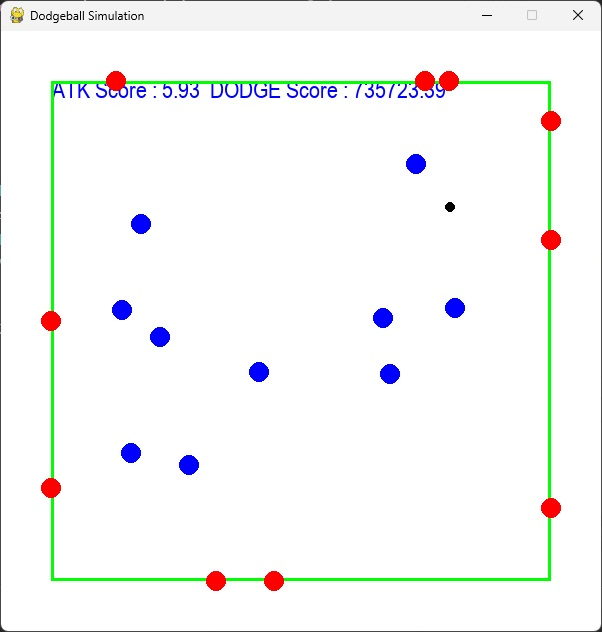
\includegraphics[width=0.5\textwidth]{images/dodgeball_demo.jpg}
    \caption{Dodgeball Game Simulation}
    \label{fig:dodgeball_demo}
\end{figure}
As shown in \xfig{fig:dodgeball_demo}, the simulation will include the following visible components:
\begin{itemize}
    \item \textbf{Game Arena:} A 2D field with defined boundaries, defined by a green rectangle.
    \item \textbf{Dodging Team:} A group of player agents colored in blue, whose primary objective is to avoid being hit by the balls. They will exhibit behaviors focused on evasion and survival.
    \item \textbf{Throwing Team:} A group of player agents colored in red, whose primary objective is to hit the dodging team with the balls. They will exhibit behaviors focused on targeting and throwing accuracy.
    \item \textbf{Ball Physics:} A simple ball, colored in black, with simulated physics, capable of being thrown by the throwing team and colliding with the dodging team.
\end{itemize}
Initialize a simple game arena with a fixed-size field and defined player locations (dodging team inside the field, throwing team outside).
Agents will receive inputs from the environment (e.g., ball position, team positions) and output actions (e.g., movement direction, throwing angle) based on their evolved strategies.

\subsection{Model and Algorithm Design}
In this project, Genetic Algorithms (GA) will be used to evolve the both teams' strategy.
Starting with simple strategies and rules, gradually increase complexity as the AI adapts, ensuring the strategies are robust and effective in a dynamic environment. The project began by focusing on the dodging team’s strategy. For the Genetic Algorithm framework, the following components will be implemented:
\begin{enumerate}
    \item \textbf{Chromosome Design:} Encode each player's behavioral parameters (e.g., movement patterns, decision thresholds) into a chromosome.
    \item \textbf{Population Initialization:} Initialize a population of strategies.
    \item \textbf{Fitness Evaluation:} Use a composite fitness function, combining factors like distance from the ball, team spacing, movement efficiency, and threat assessment.
    \item \textbf{Selection, Crossover, and Mutation:} Apply these GA operations iteratively to evolve better strategies.
\end{enumerate}
We hope to observe emergent behaviors and strategies as the dodging team evolves to survive against the throwing team, for example,
beginning with random movement, then reactive/defensive positioning, and finally threat assessment and strategic evasion. After establishing a baseline for the dodging team, introduce co-evolution by evolving the throwing team with a similar GA framework, adapting their targeting strategies.

\subsection{Parameter Tuning}

Experiment with different population sizes, mutation rates, crossover rates, and selection mechanisms to find optimal configurations.
Adjust weights in the fitness function to observe the impact on strategy development (e.g., prioritize survival vs. strategic positioning).

\section{Contributions}

\begin{enumerate}
    \item \textbf{Demonstrating Effective Use of Co-Evolution}
    \begin{itemize}
        \item Show how co-evolutionary dynamics can lead to emergent strategies in a competitive scenario.
        \item Analyze the impact of evolving two opposing forces simultaneously and how it leads to complex behavior patterns.
    \end{itemize}
    \item \textbf{Novel Fitness Evaluation in Dynamic Environments}
    \begin{itemize}
        \item Provide insights into designing effective fitness functions in competitive and dynamic environments, which can be challenging to quantify.
    \end{itemize}
    \item \textbf{Framework for Multi-Agent Strategy Simulation}
    \begin{itemize}
        \item Develop a flexible framework for simulating multi-agent systems with evolutionary computation, which can be adapted to other competitive games or simulations.
    \end{itemize}
    \item \textbf{Potential Real-World Applications}
    \begin{itemize}
        \item The project’s insights can be extended to fields requiring competitive strategy development, such as autonomous vehicles, drone coordination, or even team sports strategy analysis.
    \end{itemize}
\end{enumerate}

\section{Conclusion}
This project aims to bridge theoretical and practical aspects of Co-Evolutionary Genetic Algorithms, demonstrating their potential in creating adaptive strategies in multi-agent environments. The approach will provide a robust example of evolutionary computation applied to complex scenarios, contributing to the broader field of AI and machine learning.

\end{document}